\newpage
\subsection{The Android APP for parents}
\label{subsec:android} 

In this final subsection, we will cover the development of the Android APP. The application has been implemented alongside the advancements provided by Luca, our MID (Media \& Interaction Design) team member, who defined the overall "look\&feel" of the end result. As happened for the conjunctive work between industrial designer and soft electronics/mechanical domains, integration of the disciplines brought along unprecedented constraints. In fact, the final result we obtained required constant trade-offs between user-interaction and development feasibility. Figure \ref{fig:SE_android_overview} showcases the obtained navigability of our application, which will be covered in its main components during the upcoming pages of the report.

\begin{figure}[ht]
    \centering
    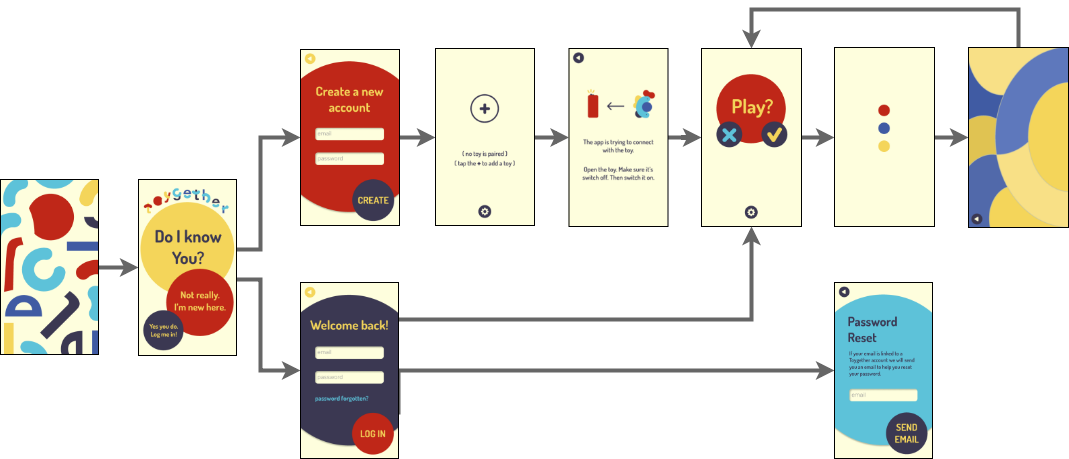
\includegraphics[scale=0.4]{images/SE_android_overview.png}
    \caption{Android app overview}
    \label{fig:SE_android_overview}
\end{figure}

\medskip
The objective of the APP, recalling the overview of the \textit{Toygether system} covered in section \ref{sec:sw}, is to fully implement a client for the parent access. To this intent, the Android APP integrates elements we previously mentioned during the development of the plush toy itself (for instance, the interactive game-play). However, the parent APP intrinsically determines a new set of challenges that are correlated with "behind the scenes" set-up taken care by the father or mother upon the first usage. In fact the parent figure, during their experience with the application, is required to, for example, both manage their personal account by procedures of log-in/log-out and provide a pairing pipeline to associate toy and parent together. This challenge has been a major discussion during the process that would design the application and its user-interaction during the different brainstorming addressing the topic.

\medskip
After illustrating how the APP was designed to best implement the client requirements (subsubsection \ref{subsubsec:android-client}), the focus will be given to two major components facilitating the pairing pipeline: the WiFi SmartConfig (\ref{subsubsec:android-smartconfig}) and the QR-code reader (\ref{subsubsec:android-barcode}). Many other functions and efforts during the implementation of the APP won't be described in detail in this report. This decision is associated with our desire to allocate major focus of the report to exploratory and implementing phases that were fundamental to the project. 

\newpage
Following the methodology we adopted to present the server (subsection \ref{subsec:server}), a stack diagram is illustrated in figure \ref{fig:SE_stack_android}. This representation is useful to underline the different dependencies between each component. Moreover, it showcases the adoption of three different libraries/API upon which the customized implementation has been built over. In particular. the Android APP has been developed with the adoption of the followings: the Java socket library \cite{javaTCPsocketDoc} for the client capability; the Barcode API by Google \cite{barcodeAPItutorial} for the QR-code recognition and finally the SmartConfig protocol \cite{smartconfigDoc} designed by EspressIf (manufacturer of the micro-controller inside the plush toy). 

\begin{figure}[ht]
    \centering
    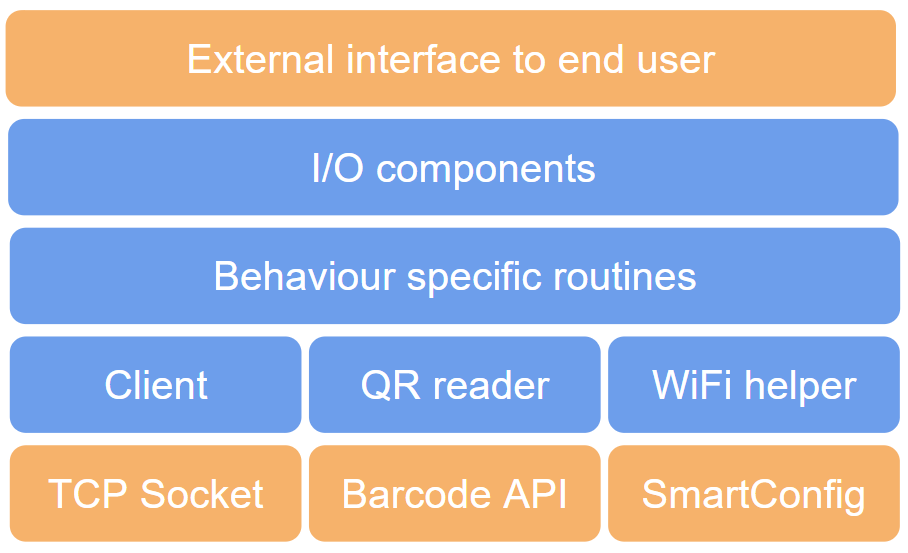
\includegraphics[scale=0.45]{images/SE_android_stack.PNG}
    \caption{Stack diagram for the Android APP dependencies}
    \label{fig:SE_stack_android}
\end{figure}

\subsubsection{A client within the system}
\label{subsubsec:android-client}

The Android APP is required to fully integrate into the \textit{Toygether system} depicted in the previous sections. Thanks to the Java standard library for TCP sockets, this operation has been able to be achieved. The development mostly encountered the same guidelines we introduced during the presentation of the server software. However, due to the usage in the Android architecture, such client component have been implemented following another famous \textit{Design Pattern} by \textcite{gamma1995design}: the \textbf{Observer} pattern.

\begin{figure}[ht]
    \centering
    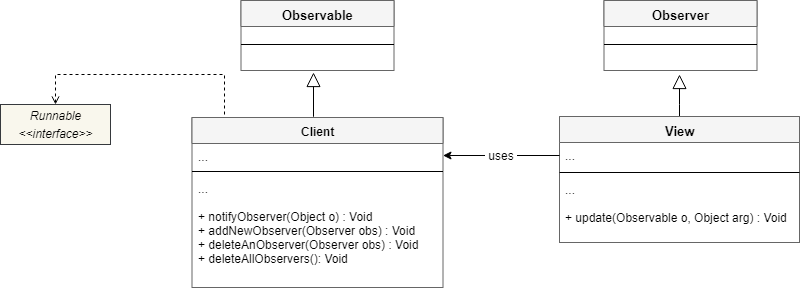
\includegraphics[scale=0.5]{images/SE_UML_android_observer.png}
    \caption{UML class diagram for the observer pattern in the Android APP}
    \label{fig:SE_UML_android_observer}
\end{figure}

Figure \ref{fig:SE_UML_android_observer} illustrates such pattern in a UML class diagram. During the execution of the application, the user is presented with a graphical user interface (GUI) that is managed by a so-called \textit{View}: a class which task is to bridge the I/O from the user with the back-end execution. In order to produce the intended result for our prototype, the application is required to trigger particular events (change colour to an element of the GUI during playing sessions) upon receiving a message from the server (MSG\_ID equal to 2003 with reference to the communication protocol in appendix \ref{appendix:messages_list}). Therefore, the \textit{View} is designed to be an \textit{Observer} with respect to the \textit{Observable} Client class. The latter, whenever a message is received, notifies such change to the whole list of \textit{Observers} (i.e. the View), which will then parse the message obtained during the automatic call of the \textit{update()} function.

\medskip
The overall implementation of the client component, as already mentioned, does not change too much from what has been introduced with the server software. The two following code-box report to the reader a simplified version (same conventions applied previously regarding try-catch clauses and output prints) of the initialisation function \textit{init()} as well as the \textit{receive()} one. One can notice that the \textit{receive()} implementation uses, as seen for the server, a Message object. Due to the multiple strength identified for such component during the server discussion, the class has been translated to be used in this context too.

\vspace{0.5cm}
\lstinputlisting[style=Java]{code_snippets/kotlin_java/android_client_init.java}
\vspace{0.5cm}
\lstinputlisting[style=Java]{code_snippets/kotlin_java/android_client_receive.java}

\subsubsection{WiFi SmartConfig for trivial connectivity setup}
\label{subsubsec:android-smartconfig} 

The project developed and illustrated in the past sections of the report depicted a connected device in detail. As we have already mentioned while describing the firmware in the subsection \ref{subsec:fw/Functions/WiFi}, the smart plush toy is connected to the \textit{Toygether system} via a WiFi connection. In order to accomplish a successful pairing with the plush toy to a parent device, one need beforehand to set-up the WiFi parameters of the toy such that it can be reached from the Android APP.

\medskip
During the section of WiFi connectivity in the firmware part (section \ref{subsec:fw/Functions/WiFi}), the so-called \texttt{SmartConfig} hot-word has been used. In fact, the real challenge that occurred for both engineering and design point of view has been to implement a pipeline for configuring the micro-controller WiFi module regardless of the limited input (no screen and keyboard for such demanding task). Thanks to the development conducted by EspressIf (manufacturer of the ESP32 micro-controller), we have been introduced to the possibility to configure WiFi details by using the Android APP itself during the first pairing process.

\begin{figure}[ht]
    \centering
    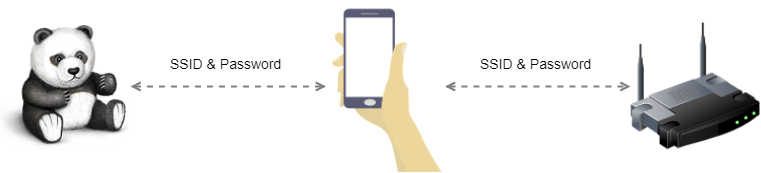
\includegraphics[scale=0.55]{images/SE_android_smartconfig.png}
    \caption{SmartConfig illustration}
    \label{fig:SE_UML_android_smartconfig}
\end{figure}

Figure \ref{fig:SE_UML_android_smartconfig} illustrates the interactions between the plush toy (on the left), the common WiFi router found in most people's homes (on the right) and the android APP itself. The goal is the ability to share the WiFi connection established on the smartphone (previously configured with the router) with the plush toy itself. Such operation is accomplished by the ESP-TOUCH protocol by \textcite{smartconfigDoc}: any WiFi enabled device (the smartphone for instance) can send UDP packets towards the WiFi access point (AP), activated by the micro-controller during this phase. Information about SSID and password of the desired network are encoded into the Length field (see diagram below) of a sequence of such UDP packets retrieved by the micro-controller.

\newcommand{\colorbitbox}[3]{%
\rlap{\bitbox{#2}{\color{#1}\rule{\width}{\height}}}%
\bitbox{#2}{#3}}
\definecolor{lightcyan}{rgb}{0.84,1,1}
\definecolor{lightgreen}{rgb}{0.64,1,0.71}
\definecolor{lightred}{rgb}{1,0.7,0.71}


\begin{center}
    \begin{bytefield}[endianness=little, bitwidth=2.4em]{16}
        \begin{rightwordgroup}{UDP packet}
        \bitbox{2}{6}
        \bitbox{2}{6}
        \colorbitbox{lightgreen}{2}{2}
        \bitbox{2}{3}
        \bitbox{2}{5}
        \bitbox{2}{Variable}
        \bitbox{2}{4}
        \\
        \bitbox{2}{\textbf{DA}}
        \bitbox{2}{\textbf{SA}}
        \colorbitbox{lightgreen}{2}{\textbf{Length}}
        \bitbox{2}{\textbf{LLC}}
        \bitbox{2}{\textbf{SNAP}}
        \bitbox{2}{\textbf{DATA}}
        \bitbox{2}{\textbf{FCS}}
        \end{rightwordgroup}
    \end{bytefield}
\end{center}

The implementation of such protocol is based on the released Android library EspressIf deployed. Thanks to such base-code, both the UDP processing and the data encryption is safely managed. On top of such functions, we have implemented and/or adapted the specific design we needed for our application in basically two classes: the first one will allow the retrieval of data like the SSID and hence covering the right part with respect to figure \ref{fig:SE_UML_android_smartconfig}; on the other hand, the second class will use the EspressIf library to define the required UDP packets with the encoded data to send.

The goal is to give to the reader a general intuition on how such classes have been used to manage a functional \textit{SmartConfig} pipeline. Firstly, the WiFi details (i.e. the SSID of the connected network for instance) need to be retrieved. The following code-boxes illustrates a few basic functions for such task.

\vspace{0.5cm}
\lstinputlisting[style=Java]{code_snippets/kotlin_java/android_smartconfig_getssid.java}
\vspace{0.5cm}
\lstinputlisting[style=Java]{code_snippets/kotlin_java/android_smartconfig_isconnected.java}
\vspace{0.5cm}

Android APIs have been fully exploited to retrieve the information about current networking details of the device. Such implementation allows the user to experience the most trivial setup possible because the information can be automatically provided. During the pairing procedure, the Android APP will require the user to be connected to the home WiFi. The only manual configuration needed will be the input of the WiFi password which cannot be done automatically for security reasons.

\medskip
As soon as the WiFi information required has been correctly retrieved, the implementation of the described ESP-TOUCH protocol can be achieved with the help of the library.

\subsubsection{QR-codes to be scanned}
\label{subsubsec:android-barcode} 

The last building block of the APP that has been explored with major importance is the QR-code reader. In fact, in the communication protocol described in subsection \ref{subsec:communication}, it has been mentioned that each client (plush toy or Android user) would be assigned an unique identifier. Moreover, each interaction is made by constructing messages whose SOURCE and DESTINATION field are only represented by such identifiers, requiring to only keep track of the server network location to function. While the pairing procedure has been already defined with a set of messages within the communication protocol, such interactions require the source client to know the identifier of the intended destination.

\medskip
The final product integrates a QR-code, like the one illustrated in figure \ref{fig:SE_qrcode}, printed on the so-called "blackbox" introduced during the previous sections. Such illustration will be the "ID card" of each plush toy joining a new household, containing all the possible details that are required to uniquely identify the client. Along with the multitude of data that can be encapsulated, the plush toy assigned identifier will be contained. The Android APP can, therefore, retrieve the toy's identifier by scanning the QR-code on the blackbox in order to construct the pairing message request (pipeline illustrated in detail during the communication protocol introduction, figure \ref{fig:SE_sequenceDiag} for reference).

\begin{figure}[ht]
    \centering
    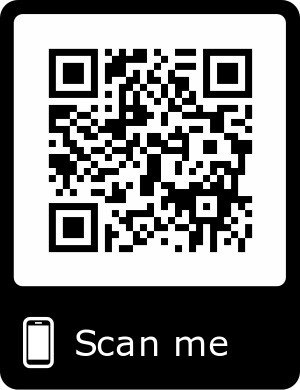
\includegraphics[scale=0.4]{images/frame.png}
    \caption{An example QR-code}
    \label{fig:SE_qrcode}
\end{figure}

\medskip
The Google Camera API from Google \cite{barcodeAPItutorial} provides a customizable set of libraries to facilitate barcode reading tasks. In particular, the API provides the correct tools to efficiently read and decode QR-code data. To this intent, the API can be invoked upon pushing a button inside the current View and running a so-called "Activity-for-result". The upcoming section \ref{subsubsec:android-activities} will draw a clear overview around the concept of Activities in Android development, but the main understanding at this phase is that the current view delegates the QR-code reading procedure to the library and halts for the result to be delivered back.

\vspace{0.5cm}
\lstinputlisting[style=Kotlin]{code_snippets/kotlin_java/android_barcode_start_intent.kt}
\vspace{0.5cm}

Invoking the Google Camera API will activate the camera interface on the Android APP, which will wait for a QR-code to be read. Once such event is triggered, the activity of task will idle and the execution focus will return to the previous one that has been halted for the results to be received back. The following function \textit{onActivityResult()} is automatically invoked in order to handle the data returned. Therefore, the method will check the correctness of the code retrieved in the scanned QR-code and subsequently share it with the next phase of the pairing pipeline. The reader needs to remember that once such code has been retrieved it will be used to communicate with the intended plush toy and accomplish the pairing procedure via the messages described previously.

\vspace{0.5cm}
\lstinputlisting[style=Kotlin]{code_snippets/kotlin_java/android_barcode_result.kt}
\vspace{0.5cm}

\subsubsection{Android Activity management}
\label{subsubsec:android-activities} 

In this final part of the Android overview, we aim to illustrate the important so-called "Activity Life-cycle". This part will be clarifying concepts about Activities introduced in the previous pages and that has been left unexplained to the reader. 

\medskip
Due to intrinsic non-deterministic execution of mobile applications (i.e. the mail APP shows the inbox view when launched from its icon, but shows the mail composition view if called by another app for instance), the coding design cannot be the same as the one usually seen on firmware (based on a main function). The code illustrated in section \ref{sec:fw} has been designed such that execution of it (turning the micro-controller ON) would deterministic-ally start at the same point every time. The Android official documentation defines activities as an object both encapsulated and focused, which provide I/O to the user (i.e. a GUI) for some result. By using activities, the Android APP is partitioned in a collection of isolated running environment, which can be directly be executed (i.e. the compose mail activity can be instantiated without passing through other parts of the code), and thus providing a correct paradigm for the application development. At the beginning of this Android-focused subsection, figure \ref{fig:SE_android_overview} illustrated the general navigability of the developed APP by showing each view. Each of such views, therefore, has been implemented in the application as an activity-object.

\medskip
Each activity inherits from the superclass a set of commonly used functions that will be helpful to handle their life-cycle behaviour later on. Appendix \ref{appendix:activity methods} provides to the reader a complete table of such methods alongside with description of their usage. Activities are usually defined with \textbf{at least} function \textit{onCreate()} and \textit{onPause()} implemented. Figure \ref{fig:SE_android_activities} on the following page illustrates how the life-cycle of activities evolves alongside the different methods used to drive the correct behaviour.

\medskip
In subsubsection \ref{subsubsec:android-client}, the observer pattern has been introduced for its usage between views and the client software. We have illustrated the possibility for a particular view (i.e. an activity according to the current discussion) in the navigability of the APP to become an \textit{Observer} of the client software. Whenever the latter would receive a new incoming message, the view would be notified of such change and receive the message to be parsed. However, we cannot give \textit{Observer} privileges to all activities at the same time for the intended application. According to the communication protocol (see appendix \ref{appendix:messages_list} for reference) once the parent has requested a playing session to the paired plush toy, the latter needs to accept it by sending a message (MSG\_ID equal to 2002) upon having the kid interacting with it. During this time, the parent is presented with a "waiting" activity until such message is not retrieved. During this period, the activity needs to be set to observe the client on hold for an interaction coming from the plush toy. As soon as the playing session is accepted, the "game" activity is proposed to the user in the foreground. In order to enable the interaction with the plush toy in both directions (sending and receiving messages for the game), this new activity needs to become an \textit{Observer} as well. However the "waiting" activity has been pushed to the background by the execution of the game and, therefore, no longer requires to observe the client. The illustrated scenario is implemented by fully exploiting the Activity Life-Cycle described, which enables the application to promptly update its behaviours on activity changes. Following the information in figure \ref{fig:SE_android_activities}, the required design is translated by correctly using functions \textit{onResume()} and \textit{onPause()} as shown in the following code-box.

\vspace{0.5cm}
\lstinputlisting[style=Kotlin]{code_snippets/kotlin_java/android_activity.kt}
\vspace{0.5cm}

\begin{figure}[hbtp]
    \centering
    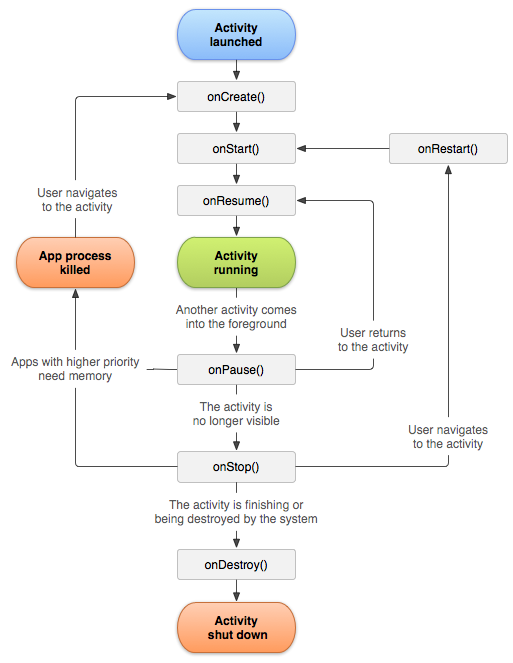
\includegraphics[scale=0.9]{images/SE_android_activities.png}
    \caption{The life-cycle of an activity in an Android APP}
    \label{fig:SE_android_activities}
\end{figure}